\newpage
\section{Introduction}
网络上绝大多少的数据是视频, 需要算法利用理解这些数据, 但视觉信息难以理解. 

\subsection{A brief history of computer vision}
\begin{enumerate}
    \item 视觉是顶尖猎杀者的通行证. 
    \item 分层的视觉感知
    \begin{figure}[!htb]
        \centering
        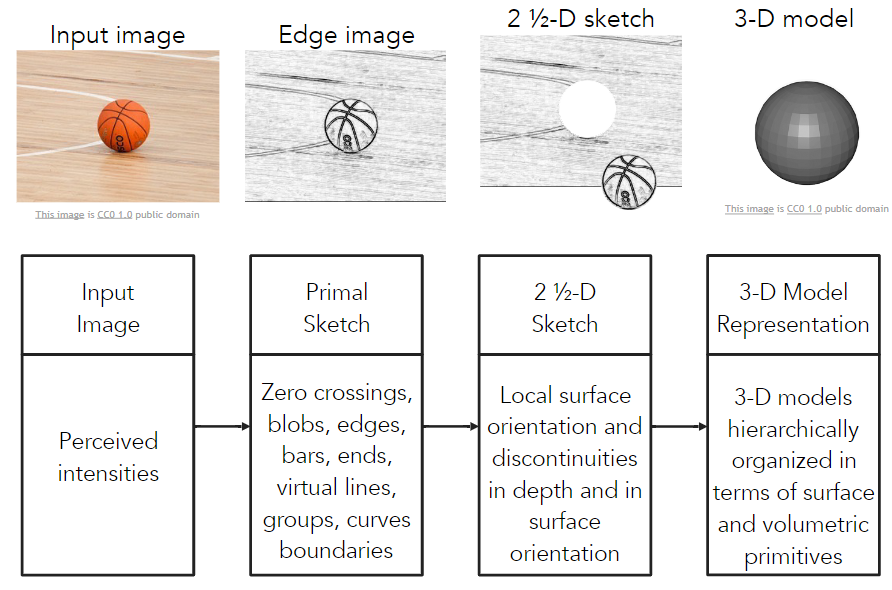
\includegraphics[width=0.42\textwidth]{pic/Lec1/Stages of Visual Representation.png}
        \caption{Stages of Visual Representation}
    \end{figure}
    \item 通过一些简单的几何结构表示世界复杂的物体. 
    \item SIFT: 特征匹配
    \item 识别小特征, 将之组合并训练识别算法
    \item 数据集: 因为数据的复, 所以需要更多的参数来拟合, 由此也需要更多的数据, 但数据也可能造成过拟合. 
    \item branch mark (基准测试). 人类的标准真的是一个人花了很多时间跑了一遍数据集, 离谱
    \item 2012 CNN deep learning
\end{enumerate}


\subsection{Overview}
Focuses on image classification

Convolutional Neural Networks (CNN) have become an important tool for object recognition. 

增大模型可以提升效果, 数据也很重要. 


